\documentclass{scrartcl}
\usepackage[utf8]{inputenc}
%\usepackage[T1]{fontenc}
\usepackage[a4paper, left=2.5cm, right=2.5cm, top=2.5cm, bottom=4cm]{geometry}
\usepackage[english]{babel}
\usepackage{amsmath, amsthm, amssymb, amstext}
\usepackage{listings}
\usepackage{color}
\usepackage{graphicx}
\usepackage{xparse}
\usepackage{fancyhdr}
\usepackage{algorithmicx}
\usepackage{algpseudocode}
\usepackage{algorithm}
\usepackage{parskip}
\usepackage[table]{xcolor}
\usepackage{tabularx}
\usepackage{enumerate}
\usepackage{enumitem}
%\usepackage{minted}
\usepackage {tikz}
\usetikzlibrary{positioning}

\pagestyle{fancy}


\rhead{{\newcommand\and\\\getauthors}}
\author{Felix Bühler\\2973410 \and Clemens Lieb\\3130838 \and Steffen Wonner\\2862123 \and Fabian Bühler\\2953320}
\lhead{\textbf\gettitle}
\title{\gettitle}
\chead{\getsubtitle}
\subtitle{\getsubtitle}

\addtolength{\headheight}{2\baselineskip}
\renewcommand{\headrulewidth}{0pt}

\newcommand{\gettitle}{Distributed systems I\\Winter Term 2019/20}
\newcommand{\getsubtitle}{G2T1 – Assignment 3 (theoretical part)}
\newcommand{\getauthors}{Felix Bühler \and Clemens Lieb \and Steffen Wonner \and Fabian Bühler}
\setlength{\headheight}{53pt}

\begin{document}
\maketitle

\section*{1 - Physical Clocks}
\subsection*{a)}

\begin{figure}[ht!]
\begin{tikzpicture}[scale=0.15]
\foreach \x in {1,...,97} {
	\draw (\x,0) -- (\x, 2);
	\draw (\x, -5) -- (\x, -7);
};
\draw (0,0) -- (97,0);
\draw (0,-5) -- (97,-5);
\node at(0, -1) {\tiny Master};
\node at(0, -4) {\tiny Slave};
\foreach \x/\n in {3/7,9/8,15/9,21/10,27/11,33/12,39/13,45/14,51/15,57/16,63/17,69/18,75/19,81/20,87/21,93/22} {
	\draw node[rectangle, fill=black, text width=1mm, inner sep=0, minimum height=3mm] at(\x + .5,1) (a\n) {}
		node[below=7mm, above of=a\n] {\tiny \n};
};
\foreach \x/\n in {3/3,9/4,15/5,21/6,27/7,33/8,37/9,41/10,45/11,49/12,53/13,57/14,61/15,65/16,69/17,73/18,77/19,81/20,87/21,93/22} {
	\draw node[rectangle, fill=black, text width=1mm, inner sep=0, minimum height=3mm] at(\x + .5,-6) (b\n) {}
		node[above=7mm, below of=b\n] {\tiny \n};
};
\path[draw,->] 
	(b5.north) edge (a10.south)
	(a11.south) edge (b8.north);
\end{tikzpicture}
\caption{Solution for Figure 1}
\end{figure}
\begin{align*}
O = \frac12((t_2 - t_1) - (t_4 - t_3)) = \frac12((10 - 5) - (8 - 11)) = \frac12(5 + 3) = 4  &\\
d = 1 & \\
\Delta = 12, C_s(t_4 + \Delta) = 20 & \\
\frac{dC_S}{dt} = \frac{12 + 4}{12} = \frac{4}{3} &
\end{align*}


\begin{figure}[ht!]
	\begin{tikzpicture}[scale=0.15]
	\foreach \x in {1,...,97} {
		\draw (\x,0) -- (\x, 2);
		\draw (\x, -5) -- (\x, -7);
	};
	\draw (0,0) -- (97,0);
	\draw (0,-5) -- (97,-5);
	\node at(0, -1) {\tiny Master};
	\node at(0, -4) {\tiny Slave};
	\foreach \x/\n in {3/1,9/2,15/3,21/4,27/5,33/6,39/7,45/8,51/9,57/10,63/11,69/12,75/13,81/14,87/15,93/16} {
		\draw node[rectangle, fill=black, text width=1mm, inner sep=0, minimum height=3mm] at(\x + .5,1) (a\n) {}
			node[below=7mm, above of=a\n] {\tiny \n};
	};
	\foreach \x/\n in {3/6,9/7,15/8,21/9,27/10,33/11,49/12,65/13,81/14,87/15,93/16} {
		\draw node[rectangle, fill=black, text width=1mm, inner sep=0, minimum height=3mm] at(\x + .5,-6) (b\n) {}
			node[above=7mm, below of=b\n] {\tiny \n};
	};
	\path[draw,->]
		(b8.north) edge (a4.south)
		(a5.south) edge (b11.north);
\end{tikzpicture}
\caption{Solution for Figure 2}
\end{figure}
\begin{align*}
O = \frac12((t_2 - t_1) - (t_4 - t_3)) = \frac12((4 - 8) - (11 - 5)) = \frac12(-4 - 6) = -5  &\\
d = 1 & \\
\Delta = 3, C_s(t_4 + \Delta) = 14 & \\
\frac{dC_S}{dt} = \frac{3}{3 +5} = \frac{3}{8} &
\end{align*}
	

\subsection*{b)}

\section*{2 - Logical Clocks}
\subsection*{a)}
\begin{enumerate}[label=(\roman*)]
	\item 
	C(e$^1_1$) = 2\\
	C(e$^2_1$) = 3\\
	C(e$^3_1$) = 4\\
	C(e$^4_1$) = 5\\

	C(e$^1_2$) = 5\\
	C(e$^2_2$) = 6\\
	C(e$^3_2$) = 7\\
	C(e$^4_2$) = 8\\

	C(e$^1_3$) = 1\\
	C(e$^2_3$) = 2\\
	C(e$^3_3$) = 3\\
	C(e$^4_3$) = 9\\
	\item 
	VC(e$^1_1$) = \texttt{[1 0 1]}\\
	VC(e$^2_1$) = \texttt{[2 0 1]}\\
	VC(e$^3_1$) = \texttt{[3 0 1]}\\
	VC(e$^4_1$) = \texttt{[4 0 1]}\\

	VC(e$^1_2$) = \texttt{[3 1 1]}\\
	VC(e$^2_2$) = \texttt{[3 2 2]}\\
	VC(e$^3_2$) = \texttt{[3 3 2]}\\
	VC(e$^4_2$) = \texttt{[3 4 2]}\\

	VC(e$^1_3$) = \texttt{[0 0 1]}\\
	VC(e$^2_3$) = \texttt{[0 0 2]}\\
	VC(e$^3_3$) = \texttt{[0 0 3]}\\
	VC(e$^4_3$) = \texttt{[3 4 4]}\\
	\item
	P$_1$: e$^1_1$ e$^2_1$ e$^3_1$\\
	P$_2$: e$^1_2$ e$^2_2$\\
	P$_3$: e$^1_3$ e$^2_3$\\
	The vector event time of those events is smaller than the vector event time of e$^3_2$. A smaller vector time means events are causally related.
\end{enumerate}
\subsection*{b)}
\begin{enumerate}[label=(\roman*)]
	\item 
	P$_1$: e$_6$ e$_5$ e$_9$ e$_4$ e$_8$ e$_{10}$\\
	P$_2$: e$_{12}$ e$_3$ e$_{13}$\\
	P$_3$: e$_{11}$ e$_7$ e$_1$ e$_2$\\
	\item 
	Local event: e$_5$ e$_9$ e$_3$ e$_1$ e$_{11}$\\
	Send event: e$_6$ e$_4$ e$_{10}$ e$_{12}$\\
	Recieve event:  e$_8$ e$_{13}$ e$_7$ e$_2$\\
\end{enumerate}

\section*{3 - Global State}
\subsection*{a)}
$ \{(e^{1}_{1}, e^{1}_{2}), (e^{2}_{1}, e^{2}_{2}), (e^{2}_{2}, e^{3}_{1}), (e^{4}_{1}, e^{3}_{2}), (e^{4}_{1}, e^{4}_{2}), (e^{5}_{1}, e^{5}_{2}), (e^{1}_{1}, e^{2}_{2}), (e^{2}_{2}, e^{4}_{1}), (e^{4}_{1}, e^{5}_{2})\} $

\subsection*{b)}
\begin{enumerate}
	\item yes, as it is a valid linearization.
	\item no, because $ e_{2}^{3} $ can not happen before $ e_{1}^{3} $
\end{enumerate}

\subsection*{c)}
\begin{figure}[!ht]
	\centering
	\begin{tikzpicture}[auto,node distance=1.5cm]
		\node[draw] (s00) {$ S_{00} $};
		\node[draw] (s10) [below left = of s00] {$ S_{10} $};
		\node[draw] (s01) [below right = of s00] {$ S_{01} $};
		\node[draw] (s11) [below right = of s10] {$ S_{11} $};
		\node[draw] (s02) [below right = of s01] {$ S_{02} $};
		
		\node[draw] (s21) [below left = of s11] {$ S_{21} $};
		\node[draw] (s12) [below left = of s02] {$ S_{12} $};
		
		\node[draw] (s31) [below left = of s21] {$ S_{31} $};
		\node[draw] (s22) [below left = of s12] {$ S_{22} $};
		
		\node[draw] (s41) [below left = of s31] {$ S_{41} $};
		\node[draw] (s32) [below left = of s22] {$ S_{32} $};
		
		\node[draw] (s42) [below right = of s41] {$ S_{42} $};
		\node[draw] (s33) [below right = of s32] {$ S_{33} $};
		
		\node[draw] (s43) [below right = of s42] {$ S_{43} $};
		\node[draw] (s34) [below right = of s33] {$ S_{34} $};
		
		\node[draw] (s44) [below right = of s43] {$ S_{44} $};
		\node[draw] (s35) [below right = of s34] {$ S_{35} $};
		
		\node[draw] (s54) [below left = of s44] {$ S_{54} $};
		\node[draw] (s45) [below left = of s35] {$ S_{45} $};
		
		\node[draw] (s55) [below right = of s54] {$ S_{55} $};
		
		\path (s10) edge node {$ e^{1}_{1} $} (s00);
		\path (s11) edge node {$ e^{1}_{1} $} (s01);
		\path (s12) edge node {$ e^{1}_{1} $} (s02);
		
		\path (s00) edge node {$ e^{1}_{2} $} (s01);
		\path (s10) edge node {$ e^{1}_{2} $} (s11);
		
		\path (s21) edge node {$ e^{2}_{1} $} (s11);
		\path (s22) edge node {$ e^{2}_{1} $} (s12);
		
		\path (s41) edge node {$ e^{2}_{2} $} (s42);
		\path (s31) edge node {$ e^{2}_{2} $} (s32);
		\path (s21) edge node {$ e^{2}_{2} $} (s22);
		\path (s11) edge node {$ e^{2}_{2} $} (s12);
		\path (s01) edge node {$ e^{2}_{2} $} (s02);
		
		\path (s31) edge node {$ e^{3}_{1} $} (s21);
		\path (s32) edge node {$ e^{3}_{1} $} (s22);
		
		\path (s32) edge node {$ e^{3}_{2} $} (s33);
		\path (s42) edge node {$ e^{3}_{2} $} (s43);
		
		\path (s41) edge node {$ e^{4}_{1} $} (s31);
		\path (s42) edge node {$ e^{4}_{1} $} (s32);
		\path (s43) edge node {$ e^{4}_{1} $} (s33);
		\path (s44) edge node {$ e^{4}_{1} $} (s34);
		\path (s45) edge node {$ e^{4}_{1} $} (s35);
		
		\path (s33) edge node {$ e^{4}_{2} $} (s34);
		\path (s43) edge node {$ e^{4}_{2} $} (s44);
		
		\path (s34) edge node {$ e^{5}_{2} $} (s35);
		\path (s44) edge node {$ e^{5}_{2} $} (s45);
		\path (s54) edge node {$ e^{5}_{2} $} (s55);
		
		\path (s54) edge node {$ e^{5}_{1} $} (s44);
		\path (s55) edge node {$ e^{5}_{1} $} (s45);
	\end{tikzpicture}
	\caption{solution for 3.c)}
\end{figure}

\newpage
\section*{4 - Snapshot Algorithm}
\subsection*{a)}

See Figure 4

\begin{figure}[!ht]
    \centering
    \begin{tikzpicture}[auto,node distance=1.5cm,event/.style={fill=black,circle, inner sep=0pt, minimum size=5pt},state/.style={draw,rectangle, red, color=red, inner sep=0pt, minimum size=5pt, minimum width=10pt}, msg/.style={-latex,thick}, marker/.style={-latex,thick,red}]
        \node[] (p1s) {\(P_1\)};
        \node[] (p2s) [below = of p1s] {\(P_2\)};
        \node[] (p3s) [below = of p2s] {\(P_3\)};
        
        \node[] (p1e) [right = 13cm of p1s] {};
        \node[] (p2e) [right = 13cm of p2s] {};
        \node[] (p3e) [right = 13cm of p3s] {};
        
        \path (p1s.east) edge (p1e);
        \path (p2s.east) edge (p2e);
        \path (p3s.east) edge (p3e);
        
        \node[event,label={\(e_1^1\)}] (e11) [right = 1.3cm of p1s] {};
        \node[event,label={\(e_2^1\)}] (e21) [right = 1cm of p2s] {};
        \node[event,label={\(e_3^1\)}] (e31) [right = 2cm of p3s] {};
        
        
        \node[event,label={\(e_1^2\)}] (e12) [right = 4.2cm of p1s] {};
        \node[event,label={\(e_2^2\)}] (e22) [right = 2.1cm of p2s] {};
        \node[event,label={\(e_3^2\)}] (e32) [right = 4cm of p3s] {};
        
        
        \node[event,label={\(e_1^3\)}] (e13) [right = 6cm of p1s] {};
        \node[event,label={\(e_2^3\)}] (e23) [right = 4.5cm of p2s] {};
        \node[event,label={\(e_3^3\)}] (e33) [right = 10cm of p3s] {};
        
        
        \node[event,label={\(e_1^4\)}] (e14) [right = 7cm of p1s] {};
        \node[event,label=below:{\(e_2^4\)}] (e24) [right = 8.5cm of p2s] {};
        
        
        \node[event,label={\(e_1^5\)}] (e15) [right = 10.5cm of p1s] {};
        \node[event,label={\(e_2^5\)}] (e25) [right = 9cm of p2s] {};
        
        \node[event,label={\(e_2^6\)}] (e26) [right = 12.5cm of p2s] {};
        
        \path (e21) edge[msg] node {\(m_1\)} (e31);
        \path (e11) edge[msg] node[left] {\(m_2\)} (e23);
        \path (e22) edge[msg] node[right] {\(m_3\)} (e12);
        \path (e32) edge[msg] node[below right] {\(m_4\)} (e14);
        \path (e13) edge[msg] node[right] {\(m_5\)} (e25);
        \path (e15) edge[msg] node {\(m_6\)} (e26);
        \path (e24) edge[msg] node {\(m_7\)} (e33);
        
        \node[state,label={[red]:{\(s_3\)}}] (s3) [right = 3cm of p3s] {};
        \node[state,label={[red]:{\(s_1,c_4\)}}] (s1) [right = 5cm of p1s] {};
        \node[state,label={[red]below:{\(s_2,c_1\)}}] (s2) [right = 6.5cm of p2s] {};
        
        \node[state,label={[red]:{\(c_2\)}}] (c2) [right = 8cm of p1s] {};
        \node[state,label={[red]:{\(c_3\)}}] (c3) [right = 8.5cm of p3s] {};
        
        \path (s3.north east) edge[marker] node[below] {\(M\)} (s1.south west);
        \path (s1.south east) edge[marker] node[left] {\(M'\)} (s2.north west);
        \path (s2.north east) edge[marker] node[below left] {\(M''\)} (c2.south west);
        \path (s2.south east) edge[marker] node[] {\(M''\)} (c3.north west);
    \end{tikzpicture}
    
    The red boxes represent where a process saves some state. A process state save is denoted by \(s_i\) and a channel state save by \(c_j\) where \(i\) is the process number and \(j\) is the channel number.
    \caption{solution for 4.a)}
\end{figure}

\subsection*{b)}

No channel received a message between the process starting recording and the first/second marker arriving. All channel states are empty sets.

\begin{align*}
    c_1 &= \{\}\\
    c_2 &= \{\}\\
    c_3 &= \{\}\\
    c_4 &= \{\}\\
\end{align*}

\end{document}
